\documentclass[10pt]{article}
\usepackage{geometry}
\usepackage{latexsym}
\usepackage{amsmath}
\usepackage{multirow}
\usepackage{url}
\usepackage[numbers]{natbib}
\usepackage{graphicx}
\usepackage{subcaption}
\usepackage{float}
\newgeometry{margin=2.65cm}

\graphicspath{{../figures/}}

\title{{\large CS224W Project Milestone} \\
  What is karma? Quantifying online influence and credibility
}
\author{Thomas Dimson \\ {\tt tdimson@cs.stanford.edu}
  \and
  Milind Ganjoo \\ {\tt mganjoo@cs.stanford.edu}
}
\date{}

\begin{document}
\maketitle

\section{Introduction}

Many online communities explicitly publicize the concept of \textit{karma} or
\textit{reputation} for users, computed as a sum of positive votes by other members of
the community. These explicit measures are often seen as proxies for more
intangible notions such as \textit{influence} (the ability of a member to
persuade others) and \textit{credibility} (the trustworthiness of the user as an
member of the community). In this paper, we describe the range of network
characteristics, interactions, and temporal factors that affect the accumulation
of karma points. Using this, we build a model that predicts karma values.

Our topic is motivated by the class content discussing how users evaluate
each other in social graphs. We wish to determine whether network properties of the 
\textit{interaction graph} can explain karma metrics. Our subsequent model 
could inform a general framework for quantifying influence and credibility
on other graphs (including those without \textit{users} as nodes).

\section{Prior Work}

Most prior literature focuses on the abstract quality of \textit{influence}.
Both \citet{bakshy2011everyone} and \citet{cha2010measuring} define
influence as the ability to generate cascades on the Twitter graph. The authors
use local feature of users (e.g.\ number of followers, number of tweets,
retweets, mentions) in order to predict the ability for users to generate
cascades.

\citet{cha2010measuring} emphasizes the topic-specificity of influence -- they challenge
the notion that there is a common set of ``influentials'' who have
broad-reaching impact on online communities. Instead, they demonstrate that for
many topics, such as political events, there are special interest groups like
bloggers and politicians that see higher retweet and mention scores than the
generally popular Twitter users.

In a very recent paper, \citet{movshovitzanalysis} consider the reputation
scheme on StackOverflow (based on upvotes and accepted answers). They 
attempt to identify expert users based on their contribution
patterns and use high reputation users for validation. The authors tried many 
techniques to improve their classifier performance including PageRank and
an SVD decomposition of their interaction graphs. Notably, they find
that PageRank does not contribute significantly to their performance
and use user features such as number of answers, questions and question-answer 
rations in their final random forest model. They are
able to achieve an Area under the Curve of 81\% when classifying users
with reputations of more than 2400.

\section{Data Collection}

In this paper, we will be focusing on two relatively large internet communities:
\textbf{Hacker News} and the \textbf{StackExchange} family of
websites. On Hacker News, users submit technology-related stories as
\textit{submissions} which other users use as an anchor to threaded discussions.
A user's \textit{karma} is computed as a sum of up-votes to their stories and
comments.  The StackExchange family of websites are question-and-answer sites
where a user will post a question and solicit answers from the community. A
user's \textit{reputation} is a weighted sum based on the number of their
questions and answers that are accepted, and whether their comments and posts
are voted as helpful by the community.

Gathering data for Hacker News came with many challenges: there is no published
dump of hacker news data, and no official API. Fortunately, the creator
of ThriftDB has created HNSearch\footnote{\url{https://www.hnsearch.com/}} as a technology
demo for his database. In addition to a public website, there is an unofficial API
supporting search queries. Although the API is limited to collecting 
only 100 recent items, we were able to circumvent this by constructing queries with limited
date ranges. Over the course of a week, we extracted JSON files for every comment,
submission and user on Hacker News by repeatedly querying the API\@. To our knowledge,
ours is the only complete dump of this data available on the internet.

Collecting data for the StackExchange family of websites was relatively easier.
An anonymized data dump of the entire series of websites is released every three
months\footnote{http://www.clearbits.net/creators/146-stack-exchange-data-dump}
in XML format. We wrote a Python script to parse the XML data and extract
relevant fields. Our initial emphasis is on \textbf{Super User}, which is a website where
enthusiasts and power users users ask questions about various aspects of
computer software and hardware. We chose this website because the data
is smaller in size since the website is new relative to Stack Overflow, the first
website in the StackExchange network. For the final report, however, we will
also include analysis on StackOverflow data.

After collecting the raw data for both datasets, we created an SQLite database
with normalized columns for all the fields. We also created an interaction graph
by collecting $(\text{replier}, \text{parent poster})$ edges and then caching
the graphs on disk as a NetworkX structure. A summary of our datasets is
available in Table~\ref{tab:graphstats}. As a final step, we divided each dataset 
into train, validation and test sets at
a 70\%/15\%/15\% split. Our milestone results are reported on our validation
set.

\section{Exploratory data analysis}

\begin{figure}[h]
\centering
\begin{subfigure}{0.49\textwidth}
\centering
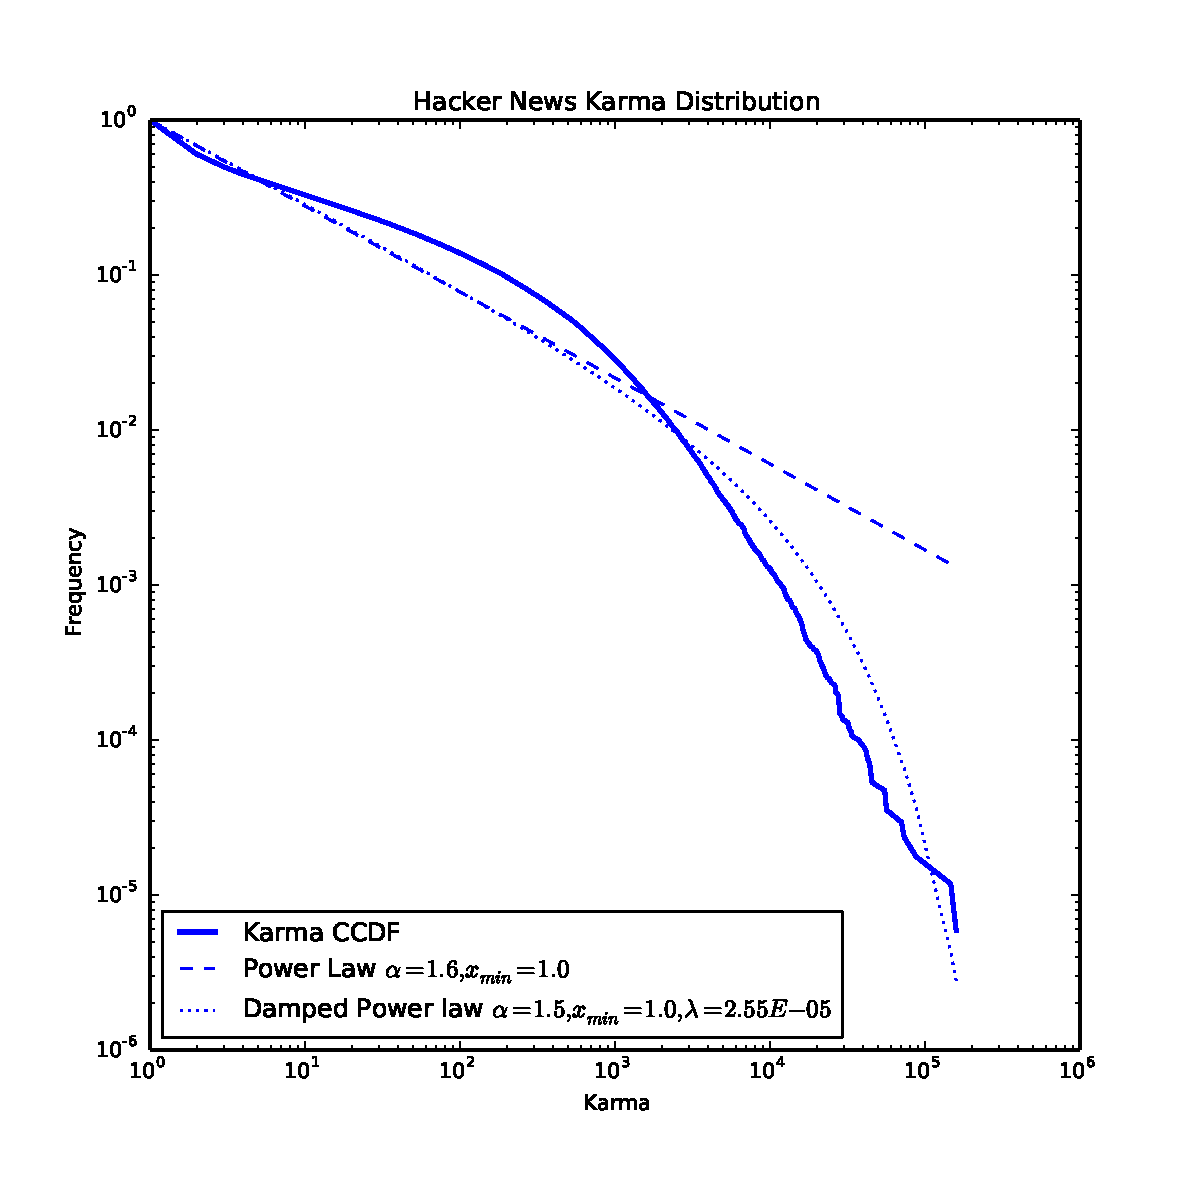
\includegraphics[width=\linewidth]{hn_karma_distribution}
\caption{Hacker News}
\label{fig:hnkarma}
\end{subfigure}%
\begin{subfigure}{0.49\textwidth}
\centering
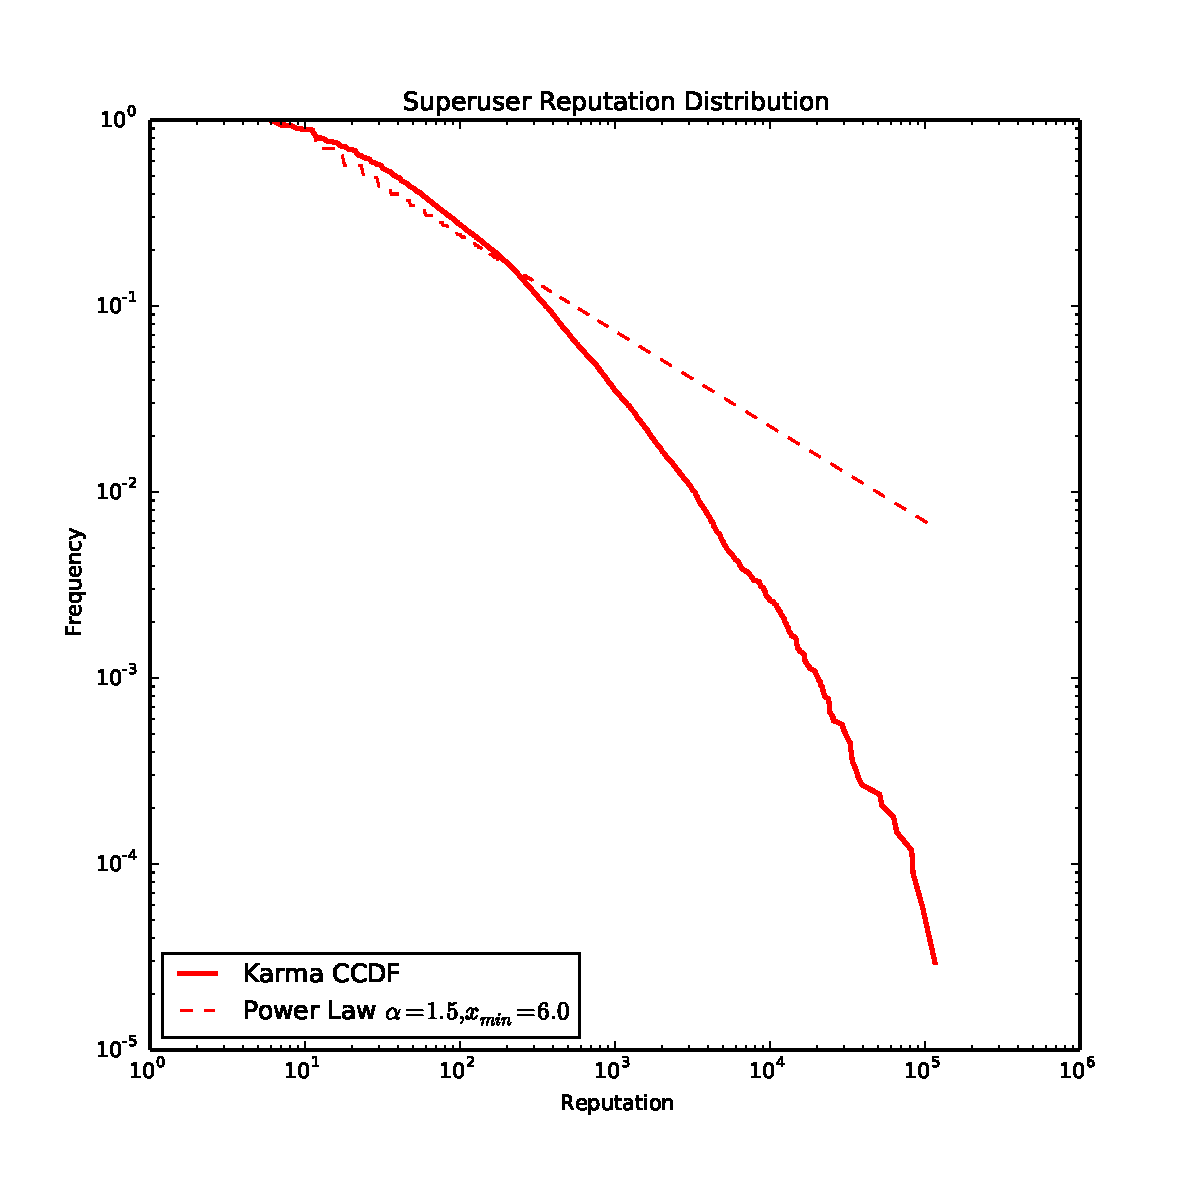
\includegraphics[width=\linewidth]{su_karma_distribution}
\caption{Super User}
\label{fig:sukarma}
\end{subfigure}
\caption{Karma distributions in our datasets with fitted power law distributions}
\label{fig:karma}
\end{figure}

We begin our data analysis with a plot of the complementary cumulative
distributions of karma and reputations over users as shown in
Figure~\ref{fig:karma}. As expected, both Hacker News and Super User
distributions are well-modelled power-law variants. Using Python's
\texttt{powerlaw} package~\cite{alstott_powerlaw:_2013} we also show fitted
models. Both models have an $\alpha$ coefficient near 1.5 and $x_{\text{min}}$
near the
origin. Notably, a damped power law is a better fit than a power law on our
Hacker News distribution and the reverse is true for our Super User reputation
distribution.  Our acting hypothesis is that Hacker News is an older community
(circa 2007) with a few early adopters with incredibly high karma while Super
User is relatively new (circa 2011) that split off of the existing StackOverflow
community.

\begin{table}[H]
\begin{center}
\begin{tabular}{| r | l l |}
\hline
& \textbf{Hacker News} & \textbf{Super User} \\
\hline
Users (Nodes) & 175091 & 190781 \\
Replies (Edges) & 2747966 & 266673 \\
Average Karma / Reputation & 131.8 & 83.1 \\
Largest SCC Fraction & 43\% & 3.8\% \\
Largest WCC Fraction & 63\% & 46\% \\
\hline
\end{tabular}
\end{center}
\caption{Graph statistics for our implied interaction graphs}
\label{tab:graphstats}
\end{table}

Aligning with our karma distributions, Table~\ref{tab:graphstats} shows
interaction graph statistics for both communities. Although they are roughly
commensurate in users, Hacker News has an order of magnitude more edges in the
graph due to the threaded nature of discussions. The disparity between the
communities increases when we begin to look at strongly connected components
(SCCs): over 40\% of Hacker News members are part of their largest SCC while
only 3.8\% of Super User members are part of their largest SCC\@. This reflects
the fact that the Q\&A site has fewer ``spanning'' conversations and a much
looser graph structure. The largest weakly connected component (WCC) is an order
of magnitude larger than the largest SCC on Super User and it suggests 
distinct roles of \textit{questioners} and \textit{answers} with
relatively little overlap. Further investigations into roles are discussed
in Section~\ref{sec:next-steps}.

For our milestone, we work on the hypothesis that \textit{karma} on Hacker News
and \textit{reputation} on Super News on these two websites are complementary
notions that can be modelled using similar intuitions. However, the differences
in graph structure revealed through exploratory analysis indicate that the
metrics may be more disparate than first thought. This is further confirmed when
we actually perform prediction in Section~\ref{sec:prediction}. In our
final report, we will use an umbrella term for the two different metrics and
highlight the aspects that are shared between them, as well as the aspects that
diverge.


\section{Predicting karma and reputation}
\label{sec:prediction}

\subsection{Regression Baseline}
Based on intuition from \citet{movshovitzanalysis}, we construct a baseline
feature matrix from the interaction graphs with two features:
\begin{itemize}
  \item the number of posts (posts, replies and comments) made by a user since
    joining the website
  \item the length of time, in seconds, since the user joined the website
\end{itemize}

\begin{table}[H]
\begin{center}
\begin{tabular}{| r | l l l l |}
\hline
&  \multicolumn{2}{l}{\textbf{Hacker News}} & \multicolumn{2}{l |}{\textbf{Super
User}} \\
Model & RMSE & $R^2$ & RMSE & $R^2$ \\
\hline
Baseline & 545.85 & 0.55 & 212.72 & 0.93 \\
Baseline+PageRank & 475.59 & 0.66 & 210.02 & 0.93 \\
Baseline+Weighted PageRank & \textbf{407.19} & \textbf{0.75} & \textbf{209.32} & \textbf{0.93} \\
\hline
\end{tabular}
\end{center}
\caption{Regression performance for our baseline and improved baseline models.}
\label{tab:regression}
\end{table}

We then perform least-squares linear regression on the set of users.
Table~\ref{tab:regression} summarizes the results of the regression. While the
root-mean-square error is not particularly helpful without a baseline, we also
include the coefficient of determination ($R^2$) which is a score in the range
$[0, 1]$ that indicates how well the points fit the regression curve.

Interestingly, we observe that the $R^2$ value for Hacker News is relatively
poor (0.5), while for Super User the regression curve fits very well (0.93). The
fact that our matrix of two baseline features fits poorly on Hacker News
indicates that karma is probably not well explained simply by how much a person
posts and how long they've been on the site. This intuitively makes sense, since
karma depends on people's \emph{perception} of a user. The reputation score, on
the other hand, is a measure of user ``authority'', and older, more active users
are likely to have high reputation simply by virtue of their status.

\subsection{Improving results with PageRank}
\label{sec:baseline-and-pagerank}
Matching the intuition that PageRank is a measure of influence, we also tried
enhancing our baseline with a PageRank feature. As illustrated in Table~\ref{tab:regression},
vanilla PageRank appears to improve performance considerably on Hacker News and have
very little effect on our Super User data. This could be explained by the large SCC
in Hacker News and is a top candidate for further exploration.

Table~\ref{tab:regression} also shows a substantial improvement
when switching from vanilla PageRank to a weighted variant. Here, we modify
our random walk so that instead of following outbound edges uniformly at random
we sample from a weighted distribution:
\begin{align}
P(i\rightarrow j)  &= \frac{\text{Num Replies}\ i \rightarrow j}{\sum_k \text{Num
replies}\ i \rightarrow k}
\end{align}
This captures the intuition that ``deeper'', multi-commented discussions
between two users are more important than one-off replies.


\subsection{Classification}
We also model the prediction task as a classification problem, where we define a
threshold for high karma and reputation on either website. Thus, we predict the
probability of a user being ``famous'' or an ``expert''.

\begin{figure}[H]
\centering
\begin{subfigure}{0.5\textwidth}
\centering
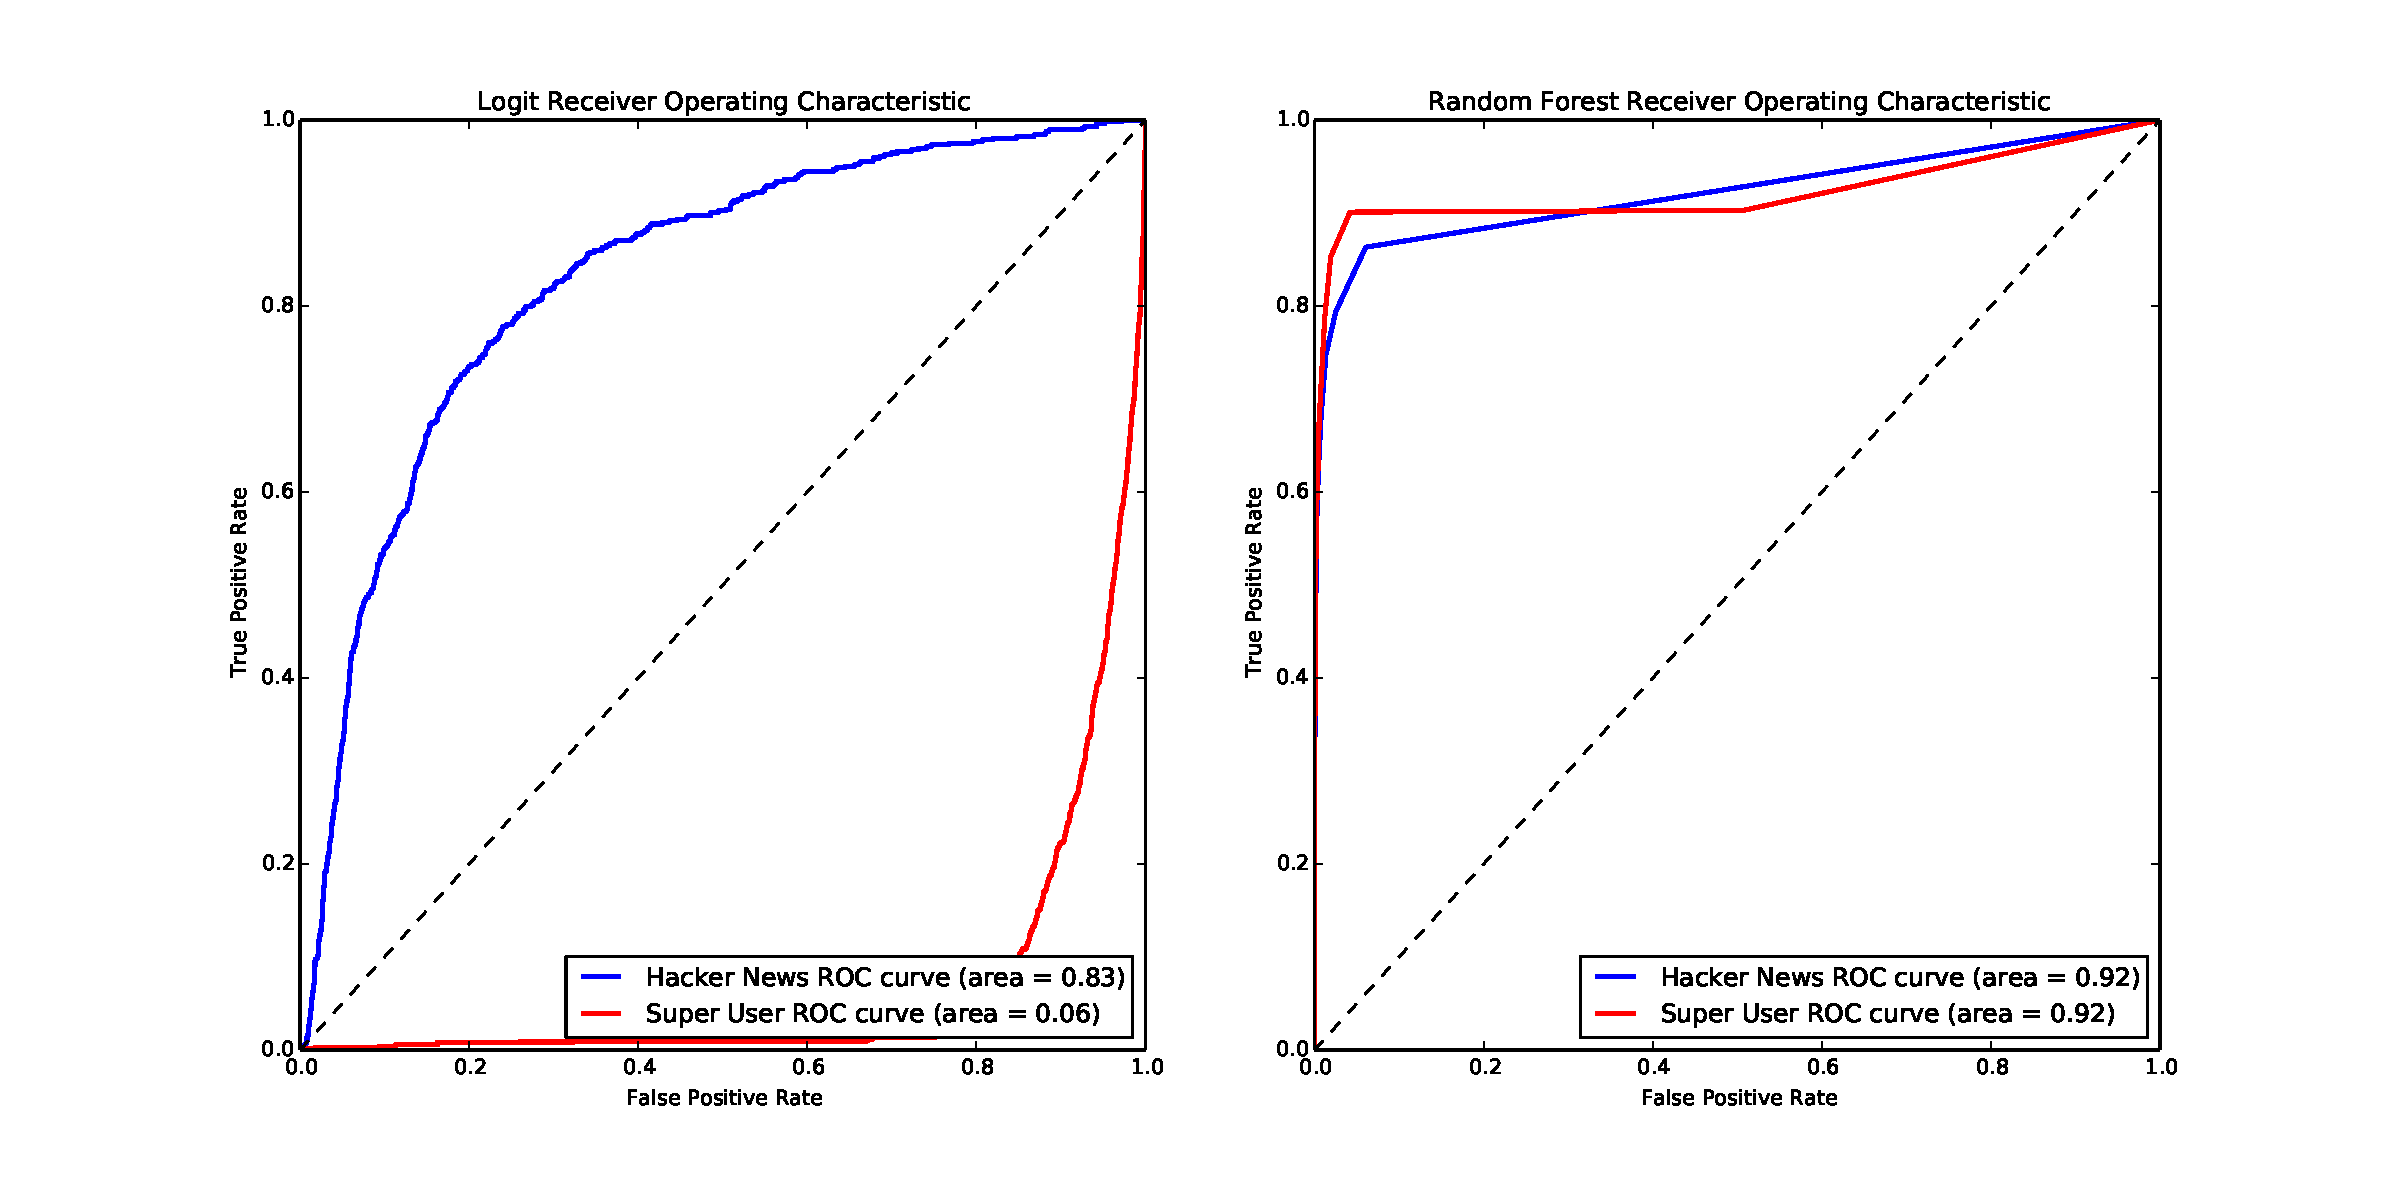
\includegraphics[width=\linewidth]{classification_roc}
\caption{ROC}
\label{fig:roc}
\end{subfigure}%
\begin{subfigure}{0.5\textwidth}
\centering
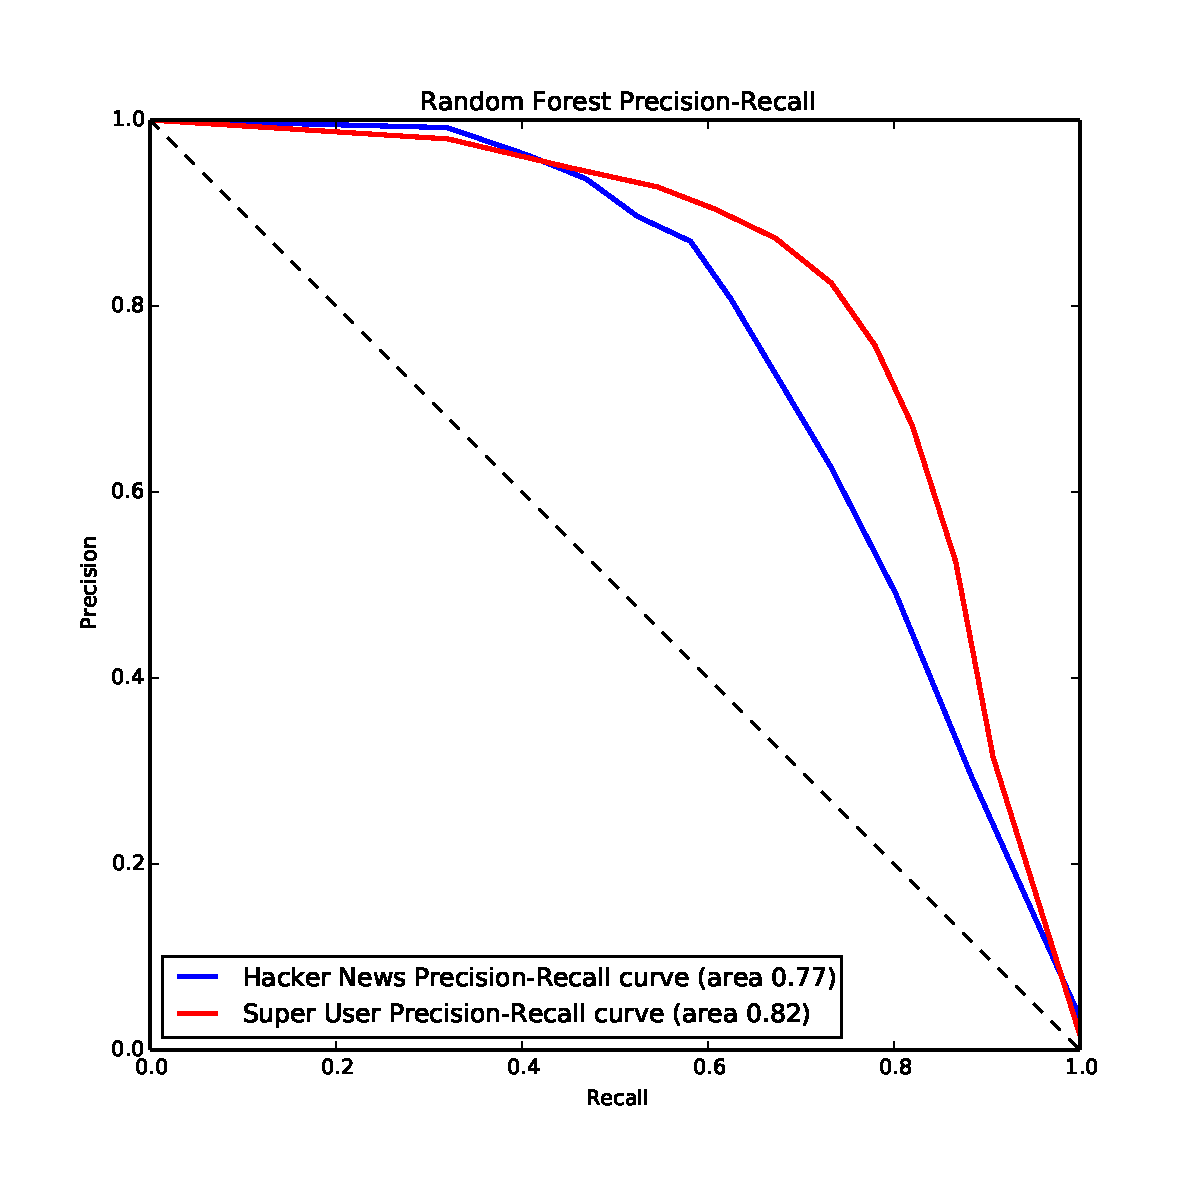
\includegraphics[width=\linewidth]{classification_pr_curve}
\caption{Precision-recall}
\label{fig:pr-curve}
\end{subfigure}
\caption{Classification performance for our improved model with weighted Page
Rank}
\label{fig:classification}
\end{figure}


For the classification task, we define a ``high karma'' user on Hacker News as
anyone with a karma above 2500, while a user with reputation above 1000 on Super
User is defined as ``high reputation''. These thresholds were defined
qualitatively based on an inspection of the karma/reputation distribution
(although we expect to formalize our choice of threshold; see
Section~\ref{sec:next-steps}). We run a logistic regression model on our dataset,
and plot the precision-recall and ROC curves. Figure~\ref{fig:classification}
shows the results for classification on our enhanced feature matrix.

The classification results for the datasets are partly consistent with the
regression results, since Super User does well in this instance also (the AUC
for the ROC curve is 0.99). On the other hand, this model does poorly on Hacker
News (even with PageRank). We believe that this is due to a bug in our Hacker News
training set which we are working to fix immediately. In any case, we
expect a better-shaped, but still poor, precision-recall curve for Hacker News
karmas.

\section{Next steps}
\label{sec:next-steps}
So far, our modeling of karma has been restricted to a few simplistic baselines.
For our final report, we anticipate coming up with a heavier, network based
explanation for karma. We are particularly interested in investigating the concept of
\emph{network constraint} to see if high-karma is associated with ``long-range''
connections. Since we are dealing with textual reply relationships, this has a natural
connection to \textit{topic modelling}. We wish to investigate whether karma
distributions are effected by the dominant topic of a user, and whether users with
relatively uniform topic distributions also have high karma. We can quantify
topics by applying Latent Dirichlet Allocation (LDA) \citep{blei2003latent}
on the comments, posts, and replies, Going deeper, we could combine our LDA-topic analysis with PageRank by
performing Topic-Sensitive PageRank \citep{haveliwala2002topic} on our nodes
and seeing if graph authority is more predictive of karma within certain
topics. This hypothesis was validated in predicting following relationships
on the Twitter graph in \citet{weng2010twitterrank}

In regards to improving classification performance, we are immediately
investigating our Hacker News data bug. Beyond that, we also believe that
we could automate the process of determining thresholds for ``high-karma''
individuals. In the limit, we can imagine using a maximum entropy classifier
to classify the karma range with logarithmic divisions.

Finally, we want to test our models and intuitions on new data. In particular, we 
will expand our Super User analysis to include \textbf{Stack Overflow}, the largest
of the StackExchange website family. Time permitting, we will also validate our
model on graphs where nodes are not \textit{users}, such as Wikipedia. It would
be particularly fascinating if karma has an intuitive meaning when applied to 
articles. 

\bibliographystyle{abbrvnat}
\bibliography{milestone}

\end{document}
